%% sudo apt-get install texlive texlive-latex-extra texlive-math-extra texlive-science texlive-fonts-recommended texlive-publishers
\documentclass[final,conference,10pt]{IEEEtran}
%\documentclass[draftcls,onecolumn,conference,12pt]{IEEEtran}
\usepackage{graphicx}
\usepackage{mathtools}
\usepackage{color,soul}

%% \date{\today}


\begin{document}

%
% paper title
% can use linebreaks \\ within to get better formatting as desired
\title{Literature Review of Embedded Software Vulnerability Protection and Mitigation Schemes}

% author names and affiliations
% use a multiple column layout for up to three different
% affiliations
\author{\IEEEauthorblockN{Nathan Palmer}
\IEEEauthorblockA{Department of Electrical and\\Computer Engineering\\
Mississippi State University\\
Starkville, Mississippi 39762\\
Email: ntp1@msstate.edu}}

\maketitle

%% References Cheat Sheet:
% {Vasserman2013,Vampire Attacks: Draining Life from Wireless Ad Hoc Sensor Networks 
% {Bojinov2010,The emergence of cross channel scripting
% {Catal2011,Software fault prediction: A literature review and current trends
% {Mahdavi-Hezavehi2013, Variability in quality attributes of service-based software system
% {Kumar2012,Implementation of Cipher Block Chaining in Wireless Sensor Networks for Security
% {Kumar2010,Classification and Review of Security Schemes in Mobile Computing
% {Singh2011,Security For Wireless Sensor Network
% {Sahoo2012,Efficient security mechanisms for mHealth applications using wireless body sensor networks
% {Aaraj2011,A framework for defending embedded systems against software attack
% {Jyostna2011,Secure Embedded System Networking An Advanced Security Perspective
% {Huang2010a,Elliptic Curve Cryptography with Security System in Wireless Sensor Networks,
% {Afreen2011,A REVIEW ON ELLIPTIC CURVE CRYPTOGRAPHY
% {Liu2012,Memory monitor module for embedded systems,
% {Mehmood2011,Incorporating Security in Embedded System–A critical analysis

\begin{abstract}
%\boldmath
Lorem ipsum dolor sit amet, consectetur adipiscing elit. Duis laoreet hendrerit luctus. Suspendisse eu libero arcu. Phasellus eu sem nec lectus semper pharetra vel fermentum nisi. Mauris sit amet turpis neque. Etiam urna nunc, viverra et dictum ac, porttitor eget elit. Aliquam rhoncus tempor sem, vitae dapibus lacus consequat dictum. Donec sit amet quam felis, at ornare augue. Fusce pretium tempor felis, imperdiet iaculis lacus egestas vel. Duis faucibus suscipit lacus, id iaculis augue rhoncus a. Cras sed nulla in arcu sodales euismod.
\end{abstract}

\section{Introduction} 

A high degree of security in embedded computer systems, specifically those used in life critical or biomedical devices, is a particularly important design goal.  Embedded systems are designed for hostile environments and operate with uniquely constrained resources. This makes embedded systems a vulnerable class of software that requires a specific set of security processes and guidelines that has not been well defined.   

There is ample research on effective software security practices for general purpose computing platforms and it is likely that many of those practices can also be applied to embedded systems. This paper provides a systematic review of recent literature related to embedded software security and general computer security trends. Issues specific to embedded software are described and prioritized based on common security risk analysis metrics.  Special emphasis is placed on wireless sensor networks and therefore literature related to low power and resource constrained wireless security will also be included.  Also, general security trends that may apply to embedded systems but seem to be under researched by the literature are presented as possible areas of future research.  The goal of this paper is to collect and report the security metrics and methods that have driven the development of secure system and application software which may also apply to embedded software.

Security researchers and practitioners can utilize these results when designing, targeting, or interfacing embedded software and platforms.  Those readers with experience in general software security practices gain perspective on where embedded systems fit into the broader security landscape.  Embedded software engineers are presented a review of security best practices and references for use during implementation.

The rest of this paper is organized as follows. Section 2, Background and Related Work, provides a background on embedded systems and the general security challenges that affect the design, implementation, and maintenance of software running on those systems. Section 3, Methodology, details the literature search, selection, and filtering process that was followed while performing this review. Section 4, Analysis and Results, contains the results of this review organized by CVSS score and reference count. Section 5, Conclusions, provides a summary of the lessons learned and includes areas for further research.

\section{Background and Related Work}
Miniaturization of computing hardware continues to drive the expansion of software into more and more areas of our lives.  This notably includes critical infrastructure, personal health, transportation devices, and diagnostic tools.  The software that resides on devices such as these provide control and communication interfaces for the underlying hardware.  The hardware that is included in these systems varies significantly between application domains but some generalizations can be made.  The diversity of targeted devices is one of the reasons why embedded software security is particularly difficult.

\subsection{Embedded Systems}

Embedded systems are characterized by tight integration and coupling with specific purpose hardware.  This is in contrast with application and system software developed for general purpose computing platforms such as racked servers or laptop and desktop computers.  Embedded software is used in cases where general purpose software is not available due to application constraints.  Typical constraints that lead to an embedded software solution are low cost, low power, and limited energy. Developing software under constraints such as these limits the resources available for security primitives such as encryption, redundancy, privilege management, and others.  Filtering specific security primitives and practices that are suitable for embedded software is an under serviced research area and one of the goals of this paper.

The following section lists some of the security related characteristics of embedded systems and software:

\begin{itemize}
\item 
Timing constraints are very tight.  Real-time operating systems (RTOS) tend to eschew security for low latency.  Many systems have custom operating systems that are written for a specific task and does not gain the benefit of a time-tested operating system.  Also, denial of service (DOS) attacks can be particularly effective due to minimum timing margins. \cite{Catal2011}
\item
Device drivers and protocol stacks are often developed in an ad-hoc and custom fashion.  This means that they may not be maintained and updated with upstream patches the way traditional systems could be.
\item 
The systems themselves are often in hostile environments. The software, hardware and interfaces are all in the attackers hands which makes reverse engineering easier than cases where the software is running on a remote server.  Embedded systems must be designed to be tamper proof to prevent modification or discovery of sensitive data.
\item 
Embedded systems tend to have low power and computing overhead which makes any security features a hard sell. Business processes may not be in place to properly prioritize software security.
Low energy, battery powered systems such as implantable or remote sensors are also subject to denial of service attacks involving energy draining.  An increase in the duty cycle of high power features could lower field life these systems. \cite{Vasserman2013}
\item 
Distributed embedded systems, such as wireless sensor networks, often operate in hostile environments where communication channels (wired and wireless) cannot be considered secure.  This necessitates encryption for command, control and communication. However, proper encryption may not be available on the embedded platform in use. \cite{Bojinov2010}
\end{itemize}

\subsection{Approaches to Embedded Security}

For many years high security was not seen as essential for these types of devices because physical barriers could be placed around the computing hardware and there were few interfaces by which a would be attacker could access the system.  This is no longer the case.  Current embedded systems require networking and configuration interfaces that are, many times, user accessible.  This is especially true for network enabled devices.  These contain many of the same vulnerabilities as traditional web servers but often lack the robust security emphasis that is afforded traditional web servers. \cite{Kumar2012}

\subsection{Wireless Sensor Networks}

Wireless sensor networks (WSN) comprise a special class of embedded system that is defined by its connectivity.  WSN devices are low power, battery powered devices that are designed to take information from their environment, perform operations on data, optionally provide feedback into the environment, and communicate with other devices.  Typically, these devices form dynamic and adaptable (ad-hoc) networks among the various sensors and may perform distributed processing on the data as well.\cite{Singh2011}  WSNs are also notable for their high profile applications such as safety critical environmental monitoring, implantable health monitoring (mHealth), perimeter security and inventory tracking.\cite{Bojinov2010,Mahdavi-Hezavehi2013,Sahoo2012}  Distributed WSN topologies are very different from traditional computer networks, such as the Internet, which tend to centralize services to specific nodes. However, this paper discusses areas of software security research that, while not originally targeted at distributed designs, can increase the security of wireless sensor networks.

\hl{[Example of embedded security breach]}

\section{Methodology}
The main goal of this study is to provide the reader with software security practices that have been reported by literature to apply well to embedded system software design and development.  However, there are several sub-goals that aid in meeting that objective.  

First, a high level study of the field is performed.  This is mainly a non-academic review of literature from trade magazines and online sources. The purpose is to gain an understanding of the field such that current trends and relevant terminology is properly included in the search methodology.

Next, the resources used for primary sources is defined.  This includes journals and databases that are used to find the raw data for analysis.  These sources are all peer-reviewed academic journals.

Following that is the creation of the search methodology.  This includes the actual search strings which are used to find journals or other articles which make up the primary sources.  Terms are chosen in an attempt to limit the search space to the overlap of software security and the environmental requirements or constraints of embedded systems.  This is an iterative step that is refined during analysis.

Once the search strings are created, the criteria for inclusion and rejection is also defined.  These criteria act as a gatekeeper to filter results such that only relevant and high quality studies are included in the analysis.

Finally, the sources which are selected for analysis are used to synthesize an authoritative list of software security practices for embedded systems.  

\subsection{Research Questions and Hypotheses}

The hypothesis this study hopes to support is that many existing software security practices can be successfully applied to embedded software to increase security in embedded systems but are not included in the literature targeting embedded system research.  The goals listed in the previous section outline the approach to confirm this hypothesis.  A further research question that is addressed is: "Where are the areas in the field of embedded software security that are high priority but under researched". The following section provides the results of some of those goals and a detailed plan for performing the final analysis.

\subsection{Current Embedded System Trends}

Current trends in embedded software development are summarised in this section in an effort to provide a context for a more thorough literature search and also to define some relevant terminology.  Most of this information was obtained from the trade publication Embedded Systems Design, the blogging portal site Embedded Gurus, and Wikipedia.  

The most obvious trend in the field of embedded systems is increased connectivity.  The so-called "internet of things" is seen by many as the next iteration of the internet. Instead of being populated by data and content entered by humans, like the current internet is, the "internet of things" is made up of physical assets that provide streams of data (environmental, biomedical, logistical, etc.) from smart sensors.  25 billion such embedded software devices are expected to be connected by 2015. Largely due to this prediction, more sophisticated networking protocols and hardware must be included on next generation embedded systems.  One example of this is IPV6 network addressing which was developed to increase the maximum number IP addressable internet nodes above 4.3 billion unique addresses.  

Another trend in embedded systems is wireless connectivity.  CPU and battery technology have progressed to the point where it is feasible to include wireless communication features to small, low power, low energy, and low cost sensors and controls.  Examples of common wireless technologies include Zigbee, Bluetooth (BTLE), and 802.11 WiFi.  Each of these protocols have specialized profiles for low energy and medical applications.

Network topologies are also an important research area for embedded systems.  Wired computer networks tend to be star, ring, or bus type networks.  However, there are advantages for wireless embedded systems that operate on mesh networks.  Specifically, a dynamically managed mesh network of wirelessly connected nodes can lead to a more robust and fault tolerant network (See \figurename \ref{fig:topology}).  Also, the network can be self-assembling.  This makes it easier to deploy networks of sensors into environments where it is difficult to predict exactly where nodes will be placed and which nodes will ultimately be connected to one another.\cite{Vasserman2013}

\begin{figure}[!t]
\centering
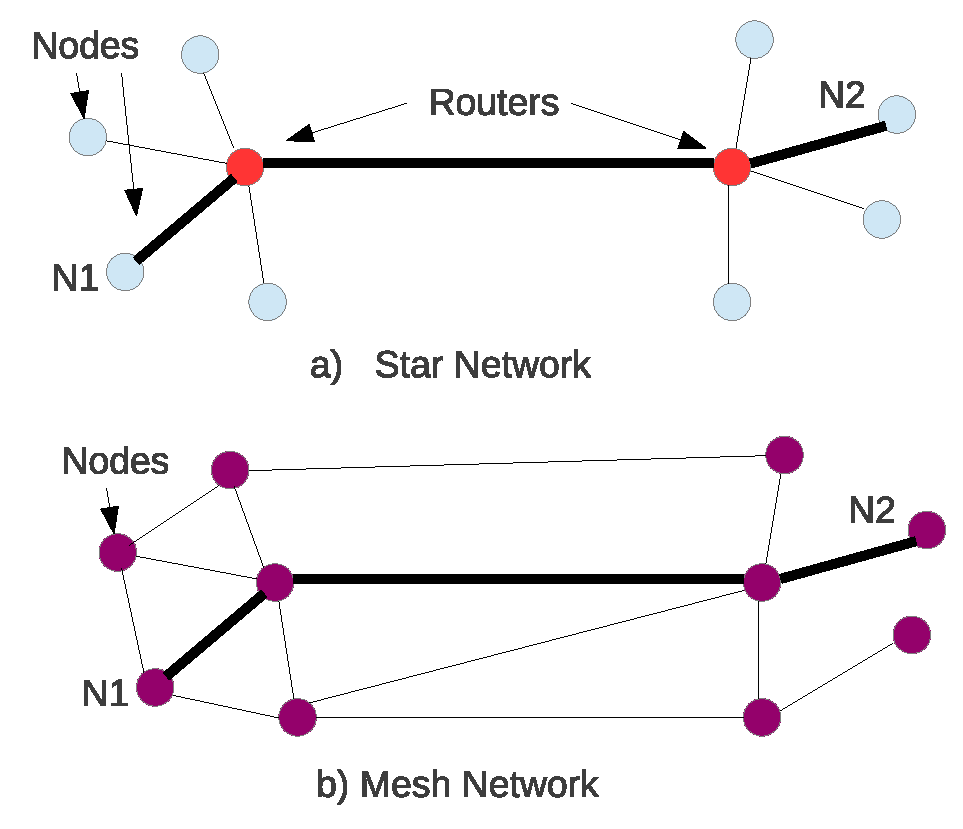
\includegraphics[width=2.5in]{topology}
% where an .eps filename suffix will be assumed under latex, 
% and a .pdf suffix will be assumed for pdflatex; or what has been declared
% via \DeclareGraphicsExtensions.
\caption{bus topology image here}
\label{fig:topology}
\end{figure}

Another trend in embedded system design is to include field upgradeable firmware.  Along with connectivity comes the desire to provide updates and patches to deployed embedded software (firmware).  This functionality can apply to individual applications and features or to the entire software suite on the device, including device drivers and system software.  Depending on the implementation, updates may require user intervention or may be pushed to the device from a vendor.  Ensuring the integrity of field installed firmware is an active area of research.

Traditionally, the majority of development for embedded software was done in low-level languages such as C or in architecture specific assembly code.  While these languages are still dominant, there is a trend towards using higher level languages for all but the lowest level functionality.  Some popular languages taking a foothold in embedded software development are Embedded Java and Embedded C++. Features such as type safety and garbage collection are new to many embedded software engineers.

Consolidation of functionality is another feature of emerging embedded systems.  Many embedded systems consist of a single system-on-a-chip (SoC) that includes not only the CPU, RAM and ROM components, but interface hardware as well.  Many include hardware for efficient network connectivity such as WIFi, Ethernet, NFC/RFID, cellular and Bluetooth physical layer devices.  Also popular are USB layer hardware, encryption accelerators, analog to digital converters, and digital signal processing (DSP) hardware. 

\subsection{Traditional Embedded System Features}

Many traditional features of embedded systems continue to affect current software design and implementation.  A reduced energy budget continues to be a constraint for battery powered devices and leads to other constraints such as low processor clock speeds and reduced system memory.  Less processing power reduces options for for security features such as encryption.  Also, it continues to be difficult to provide general purpose embedded software because the code is heavily dependent on the underlying CPU platform.  Platforms can vary in memory architecture, word size, instruction set, floating point support, and register sets.  Real-time performance (guaranteed bounds on latency) constraints are still a requirement of many embedded systems. Finally, debugging and testing is complicated by the lack of an underlying general purpose operating system and the sensitivity of the system to timing variations.  It often requires the use of sophisticated software emulators and simulators.  Often specialized hardware is also required to debug or profile the system.

\subsection{Primary Sources}

Peer reviewed journals provide the raw data for the analysis included in the following section of this paper, Section 4.  Access to the EBSCO Host database provides the searching capability utilized to find candidate papers.  All peer reviewed journals are included in the search space, but the publication date is limited to the years 2009 through 2013.

Two sets of search results are included for analysis: embedded software security specific articles and general software security articles filtered by key constraints.  The following search criteria provide the articles under review. 

\textit{Embedded Systems Software security}

Find Articles where the abstract contains:
\begin{center}
(embedded AND software) AND (security OR secure) AND (metric OR protect OR attack OR vulnerability)
\end{center}

\textit{General Software Security with Constraints}

Find Articles where the abstract contains:
\begin{center}
software AND (security OR secure) AND ("real-time" OR mesh OR "low power") NOT (embedded)
\end{center}

\subsection{Selection / Rejection Criteria}

Literature returned by the previous search criteria is further filtered based on the relevance of its results to the research questions defined above.  For the \textit{Embedded Systems Software Security} results this process is accomplished by reading the abstracts and selecting any papers that show improved security due to novel protection schemes. For the \textit{General Software Security with Constraints} results, the papers are filtered by reading the abstract and comparing the scope of the study to embedded system criteria and trends as they are described earlier in this section. Any papers that show relevant protection schemes are included in the final analysis.

\subsection{Analysis Methodology}

Each paper that is selected in the previous step is analysed for protection schemes and vulnerabilities.  A table of vulnerabilities is included in the analysis section that includes a brief description and the number of unique papers that reference the vulnerability. A score is assigned to each vulnerability that represents its relative impact to system security. The score is based on the Common Vulnerability Scoring System (CVSS) defined by the National Institute of Standards and Technology\footnote{See http://nvd.nist.gov/cvss.cfm for more information on the NVD Common Vulnerability Scoring System Support V2}.  Any protection or mitigation schemes that are reported in the literature under review are provided for the applicable vulnerabilities listed in the table.  

\section{Analysis and Results}

\subsection{Embedded Software Vulnerabilities}

Table \ref{tab:vul_summary} gives a representative list of vulnerability types found in the current literature.  The types are defined as follows.  System software attacks are those that exploit a weakness in the underlying operating system or device drivers.  This could be an upstream flaw that affects all instances of the operating system or it could be specific to the particular implementation. Application software attacks exploit weaknesses in the application specific code.  Side channel attacks are those that utilize communication channels that are not intended for communication.  Interface attacks exploit vulnerabilities in external interfaces such as USB and TCP/IP protocols, data collection inputs, or external memory interfaces.  Finally, software modification attacks change program instruction or data memory either partially or wholly to change the behaviour of the system.  The following sections go into more detail on each of the attack types and provide mitigation advice based on the current literature.

\begin{table}[!t]
%% increase table row spacing, adjust to taste
\renewcommand{\arraystretch}{1.3}
% if using array.sty, it might be a good idea to tweak the value of
% \extrarowheight as needed to properly center the text within the cells
\caption{Summary of Vulnerabilities}
\label{tab:vul_summary}
\tiny
\centering
\begin{tabular}{ | l | l | l | l | }
\hline
 Vulnerability Type & Refs & CVSS Parameters & Score \\ \hline
 Sys. Software Attack	& 3 &	\verb|AV:L/AC:H/Au:S/C:C/I:C/A:C| 	& 6		\\ \hline
 Software Modification	& 5 &	\verb|AV:L/AC:H/Au:S/C:C/I:C/A:C|	& 6		\\ \hline
 Interface Attack		& 3	&	\verb|AV:L/AC:H/Au:N/C:N/I:C/A:C|	& 5.6	\\ \hline
 Cross Channel Attack	& 1 &	\verb|AV:N/AC:H/Au:S/C:P/I:P/A:P|	& 4.6	\\ \hline
 App. Software Attack	& 4 &	\verb|AV:L/AC:M/Au:S/C:P/I:P/A:P|	& 4.1	\\ \hline
 Side Channel Attack		& 3 &	\verb|AV:L/AC:H/Au:N/C:C/I:N/A:N|	& 4		\\ \hline
\end{tabular}
\end{table}

\subsubsection{System Software Attacks}
System software controls access to hardware resources through memory management and/or device drivers.  It also arbitrates access to the processor by allocating time slices for processes.  Many embedded system developers will write custom system software to access custom hardware or to meet strict real-time requirements. There are also operating systems that are written specifically for embedded systems.  Flaws in these systems can be exploited by malicious users to compromise an embedded system.  

Attacks on system software can be carried out by exploiting traditional weak links in software design, such as buffer overflows or direct memory modification.  However, because system software tends to run with elevated privilege and has direct access to memory, vulnerabilities are more dangerous than in application software.  

Mitigation strategies suggested by the literature bypass the system software.  One approach is to encapsulate integral security software, such as encryption or authentication methods, in secure memory and only access through special hardware separated memory.\cite{inveos}  This allows some assurance of the integrity of the system, while still allowing the use of a monolithic OS.  Note that these approaches require hardware monitoring of the secure memory because it is assumed that if the system software is compromised then the attacker has full read and write access to the system's memory.

Another approach to this problem is to include a separate operating system for security critical processes.  A custom micro-kernel could be included to provide security related functionality to the system.  This OS could execute in parallel with the main OS using hardware memory separation or it could have it's own independent memory space and communicate though a secure bus.\cite{novelOS}

\subsubsection{Application Software Attacks}

Application code is another area of attack in embedded systems.  Exploits on application code may not compromise the entire system like system software does, but it can reveal sensitive information or compromise specific system functionality.  Application code can be attacked with injected code or buffer overflow attacks, among others.  The literature seems to focus on two mitigation approaches to application attacks: detection and prevention.  

Attacks can be detected using static code analysis.  The expected number of instructions or clock cycles between specific checkpoints in the code can be determined at compile time and monitors (hardware or software) can ensure that the expected number of clock cycles or instructions were actually executed.  A discrepancy indicates that the code was modified.  Prevention of such attacks can be implemented via program and data encryption.  The program instructions can be encoded using an encryption scheme that ensures that modifications are detected.  The instructions are decoded by the processor at execution time.  Modification of the code results in invalid processor instructions. \cite{compiler-hardware} \cite{architectural-frameworks}

\subsubsection{Side Channel Attacks}
Side channel attacks are those that utilise interfaces to the device that are not intended for communication such as power supply, electromagnetic, or acoustic channels.  Many papers have shown that careful analysis of timing, electromagnetic emissions, or energy consumption can reveal the internal state of an embedded system. \cite{papers??} This can be exploited to discover key features of an embedded system such as encryption algorithms and even private keys.  Power analysis attacks are a very active area of research.  Power analysis attacks sample the instantaneous current flowing into the hardware (e.g. security co-processor containing an encryption private key) during various inputs.  The patterns formed in the power analysis can be used to guess the number of rounds used an TripleDES implementation, for example.  Also, differential analysis can be performed by creating a template signal that is based on an known state.  Comparisons are made to this template to determine the value of unknown states.  

\begin{figure}[!t]
\centering
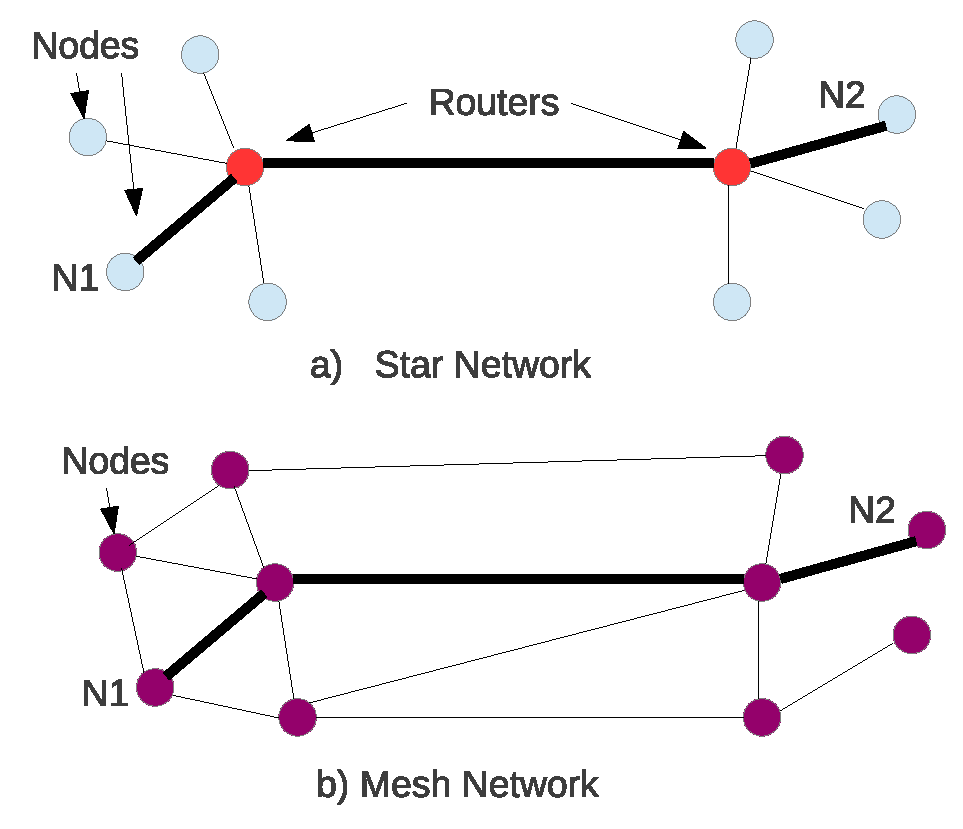
\includegraphics[width=2.5in]{topology}
% where an .eps filename suffix will be assumed under latex, 
% and a .pdf suffix will be assumed for pdflatex; or what has been declared
% via \DeclareGraphicsExtensions.
\caption{side channel image here}
\label{fig:side_chan}
\end{figure}

The effectiveness of such attacks can be mitigated in two ways: masking and hiding.  Masking the side-channel signal is accomplished by inserting random instructions to mask the signal in random noise.  Hiding works by providing a consistent, one that does not change with the state of the software, view of the system to an attacker via specialised hardware such as dual-rail pre-charge (DRP) logic gates.\cite{papers??}

\subsubsection{Cross Channel Attacks}
Cross channel attacks exploit a flaw in one communication channel to expose a vulnerability in anther channel.  This is not specific to embedded systems, but they are particularly vulnerable.  Many embedded systems use a collection of third-party software to enable networking features for services such as media access, web based configuration, wireless device discovery, etc.  Due to constraints on embedded systems, these services may have to share resources such as memory or disk space.   An vulnerability in one service, such as an open FTP user account, can lead to other attacks, such as inserting malicious Java Script code onto a device configuration website.  This is very similar to a cross site scripting attack.

There is no specific protection against this class of attacks.  However, most of the exploits that fall in to this category also exist on desktop and server platforms, so traditional security advice applies.  Input from all channels should be sanitized to protect against buffer overflow attacks and code injection.  Also, if possible, include the ability to patch any third party applications with security updates. \cite{emerge ccs paper}

\subsubsection{Interface Attacks}
Interface attack are those that exploit some weakness in the external interface of a device.  Embedded systems do not typically have screens and keyboards like personal computers and many do not have a network interface but there is always an interface to the environment.  

Some devices monitor sensors via probes that measure electrical values such as voltages and provide feedback to actuators such as motors or solenoids. An attacker can carefully craft an electrical signal to inject arbitrary values through input probes.  This approach can be used to perform buffer or integer overflow attacks.  Data sanitization should be applied to these types of inputs.\cite{Jyostna2011} 

Another interface common to embedded systems is external memory.  Data stored on a separate chip from the processor is exposed to eavesdropping on the memory interface bus.  This is commonly exploited to capture encryption keys during private key exchange or distribution.  Sensitive data should never be passed un-encrypted across an external bus, especially private keys.  Encryption and decryption should only be performed on the device that needs access to the sensitive data.\cite{off chip memory}

Finally, the Universal Serial Bus (USB) is a ubiquitous interface for embedded systems.  These ports allow high throughput data transfers to and from the device and also allow control via USB keyboards and mice.  However, the USB protocol stack is very complicated and there are many know exploits for USB drivers.  Many times these drivers run with elevated privilege allowing code injection from USB attacks to cause substantial damage.  The best way to mitigate this attack is to only provide user level USB support without elevated privilege. \cite{USB}

\subsubsection{Software Modification}
Field updates to firmware is a powerful feature and can be used to increase the security of a system by patching vulnerabilities as they are discovered.  However, having the ability to change the code running on an embedded system should be weighed against the risk of an attacker modifying the firmware to execute arbitrary code. This type of attack is common in consumer electronics (e.g. digital cameras and TCP/IP routers)  where features are enabled on lower end models that were only intended for high end versions.  Smart-phones and set-top boxes are also common targets where attackers remove key security checks from vendor's firmware and release the 'patched' versions.

Protections against software modification focus on securing the software that loads the firmware into memory to begin execution.  This boot loader should ensure that the code it is loading is unmodified or digitally signed to ensure the integrity of the instructions and data. Another option is to only allow parts of the firmware to be writeable and keep critical program code in read only memory (ROM). Finally, code can be analysed at runtime to ensure that the code is not modified after being loaded into memory.  This can be done with special hardware that counts instructions or CPU cycles between check points in the program flow to ensure that instructions were not added or removed. \cite{compiler-hw approach,fpga-based}

\subsection{General Software Security Trends}

This section explores some of the recent trends in software security that have been shown to apply to low power and wireless mesh networks systems. These trends also apply to many embedded systems and are included here to provide stimulate research in specific applications to embedded systems.

Fifty seven (57) papers were discovered using the search methodology described in the previous section.  From those, a total of twenty-nine (29) papers were analysed to compile the following list of topics, summarised in table \ref{tab:trend_summary}.  The first column names the category and the second column give the corresponding number of recent papers that focused on that topic. Literature was discarded if the abstract did not indicate an actual application to embedded systems.  The trend categories are intentionally broad to emphasize areas that are under researched. The following sections detail  the trends and how they apply to embedded systems.

\begin{table}[!t]
%% increase table row spacing, adjust to taste
\renewcommand{\arraystretch}{1.3}
% if using array.sty, it might be a good idea to tweak the value of
% \extrarowheight as needed to properly center the text within the cells
\caption{Summary of General Software Security Trends}
\label{tab:trend_summary}
\centering
\begin{tabular}{ | l | l | }
\hline
 Software Security Trend & Reference Count \\ \hline
 Security Model Checking			& 7	\\ \hline
 Encryption						& 5	\\ \hline
 Real-Time Security Monitoring	& 6	\\ \hline
 Securing Data Channels			& 3	\\ \hline
 Data Integrity					& 3	\\ \hline
 Virtualization					& 2	\\ \hline	
 Other							& 2	\\ \hline
\end{tabular}
\end{table}

\subsubsection{Security Model Checking}
Models that represent algorithms and software specifications can be created by designers using formal logic.  If the models are complete then equivalence can be verified between the specification and the algorithm. Code can also be checked against the model to prove that it properly meets the specifications.  This type of checking is difficult due to the effort involved in creating and maintaining the formal models but it is necessary for high assurance software.  Such model checking is a heavily researched area of computer science.  

Software faults are discovered in the algorithmic models before they can affect actual systems.  Model checking can be a powerful tool against malicious attacks because these faults can easily lead to security vulnerabilities.  Models can be created for the entire system or of only critical subsystems such as encryption algorithms.  Communication protocols and other interfaces can be modelled and simulated "attacks" can be performed on the models.   \cite{Probabilistic Attack Scenarios to Evaluate Policies over Communication Protocols}

Security models for embedded systems software (including specific time constraints and physical features) and attacks should be researched.

\subsubsection{Encryption}
Encryption is the standard software solution to ensuring confidentiality and often for providing integrity.  Embedded systems are highly susceptible to attacks on confidentiality of data because they tend to be small, mobile, and often physically accessible to attackers.  However, the resource limitations of embedded systems prevents the use of encryption for many applications. 

Technologies such as security coprocessors provide hardware solutions by providing specialized cryptographic accelerators for common algorithms such as DES and Elliptical Curve Cryptography (ECC).  ECC is particularly attractive to embedded systems because it requires fewer instructions than comparably secure algorithms.  

More research is necessary to develop encryption techniques that are applicable to embedded systems.

\subsubsection{Real-Time Security Monitoring}
Many attacks can be detected by their side effects to the affected system.  Malicious code, such as viruses and worms can often be detected by their signatures, of specific strings of data that are contained in their code or data.  On desktop systems, virus scanners can scan memory and disk space for the presence of malicious code.  Other, more reactive types of analyses can be performed using forensic software that looks for signs of an attack in logs or system data.  

These types of monitoring approaches could also apply to embedded system software.  Software similar to a virus scanner could scan firmware for changes indicative of an attack.  This could be a much different signature than in a desktop system, so more research is necessary.  However, some work has been done on wireless area network (WAN) monitoring that is applicable to embedded systems. \cite{}

\begin{figure}[!t]
\centering
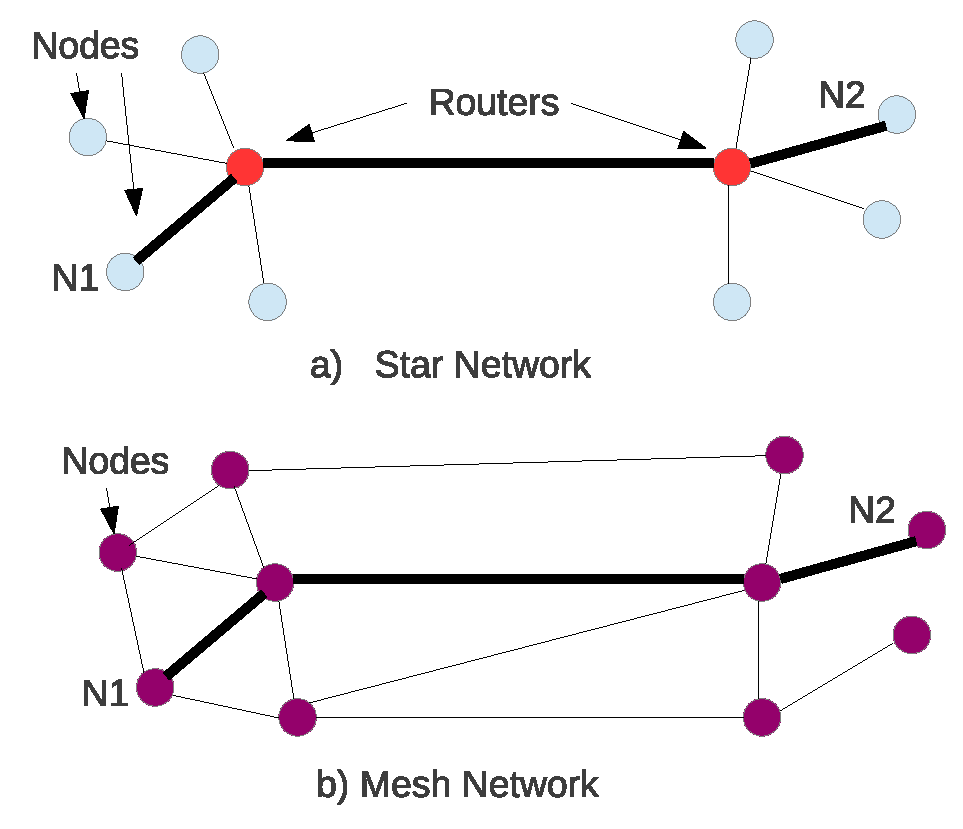
\includegraphics[width=2.5in]{topology}
% where an .eps filename suffix will be assumed under latex, 
% and a .pdf suffix will be assumed for pdflatex; or what has been declared
% via \DeclareGraphicsExtensions.
\caption{bus topology image here}
\label{fig:monitor}
\end{figure}

Embedded systems could be analysed for anomalies in behaviour by external or redundant systems.  Anomalies could manifest as behaviour that original specifications did not intend or could include checks for incorrect states, such as valves in the open and closed position at the same time or several neighbouring systems having drastically different times of temperatures. \cite{Master Failure Detection Protocol in Internal Synchronization Environment} 

\subsubsection{Securing Data Channels}
Embedded systems suffer from the same types of issues as other computing systems when they communicate in networks over hostile communication channels.  Vulnerabilities in common IP routing or framing protocols apply to embedded systems if the protocols are in use on the network.  Some technologies that are common for wireless mobile networks such as 802.11 WiFi, DSDV (Destination sequenced distance vector), WRP (Wireless Routing Protocol) are also common in embedded systems. Attacks on these protocols should be understood by embedded developers that utilize them. 

Also, issues such as key distribution in wireless networks applies to embedded networks as well.  Research on secure private key distribution in distributed networks is ongoing and should be expanded to include issues specific to embedded systems.

\subsubsection{Data Integrity}
Software integrity refers to the level of confidence that data and code have not been modified unintentionally.  Much research has been done ensuring data integrity in software.  Digital signatures are the standard technology for ensuring integrity. However, the same embedded system limitations that create problems for encryption also affect digital signatures.  

External hardware such as trusted platform modules (TPM) can be applied to embedded systems to enable digital signature verification on executed code.  This technology is used by PCs to ensure the integrity of the system BIOS and some operating systems also use it to verify critical code.  

\subsubsection{Virtualization}
Lorem ipsum dolor sit amet, consectetur adipiscing elit. Duis laoreet hendrerit luctus. Suspendisse eu libero arcu. Phasellus eu sem nec lectus semper pharetra vel fermentum nisi. Mauris sit amet turpis neque. Etiam urna nunc, viverra et dictum ac, porttitor eget elit. Aliquam rhoncus tempor sem, vitae dapibus lacus consequat dictum. Donec sit amet quam felis, at ornare augue. Fusce pretium tempor felis, imperdiet iaculis lacus egestas vel. Duis faucibus suscipit lacus, id iaculis augue rhoncus a. Cras sed nulla in arcu sodales euismod.

Lorem ipsum dolor sit amet, consectetur adipiscing elit. Duis laoreet hendrerit luctus. Suspendisse eu libero arcu. Phasellus eu sem nec lectus semper pharetra vel fermentum nisi. Mauris sit amet turpis neque. Etiam urna nunc, viverra et dictum ac, porttitor eget elit. Aliquam rhoncus tempor sem, vitae dapibus lacus consequat dictum. Donec sit amet quam felis, at ornare augue. Fusce pretium tempor felis, imperdiet iaculis lacus egestas vel. Duis faucibus suscipit lacus, id iaculis augue rhoncus a. Cras sed nulla in arcu sodales euismod.

\subsubsection{Other}
Lorem ipsum dolor sit amet, consectetur adipiscing elit. Duis laoreet hendrerit luctus. Suspendisse eu libero arcu. Phasellus eu sem nec lectus semper pharetra vel fermentum nisi. Mauris sit amet turpis neque. Etiam urna nunc, viverra et dictum ac, porttitor eget elit. Aliquam rhoncus tempor sem, vitae dapibus lacus consequat dictum. Donec sit amet quam felis, at ornare augue. Fusce pretium tempor felis, imperdiet iaculis lacus egestas vel. Duis faucibus suscipit lacus, id iaculis augue rhoncus a. Cras sed nulla in arcu sodales euismod.

Lorem ipsum dolor sit amet, consectetur adipiscing elit. Duis laoreet hendrerit luctus. Suspendisse eu libero arcu. Phasellus eu sem nec lectus semper pharetra vel fermentum nisi. Mauris sit amet turpis neque. Etiam urna nunc, viverra et dictum ac, porttitor eget elit. Aliquam rhoncus tempor sem, vitae dapibus lacus consequat dictum. Donec sit amet quam felis, at ornare augue. Fusce pretium tempor felis, imperdiet iaculis lacus egestas vel. Duis faucibus suscipit lacus, id iaculis augue rhoncus a. Cras sed nulla in arcu sodales euismod.

\section{Conclusions}

Put conclusions here....

Lorem ipsum dolor sit amet, consectetur adipiscing elit. Duis laoreet hendrerit luctus. Suspendisse eu libero arcu. Phasellus eu sem nec lectus semper pharetra vel fermentum nisi. Mauris sit amet turpis neque. Etiam urna nunc, viverra et dictum ac, porttitor eget elit. Aliquam rhoncus tempor sem, vitae dapibus lacus consequat dictum. Donec sit amet quam felis, at ornare augue. Fusce pretium tempor felis, imperdiet iaculis lacus egestas vel. Duis faucibus suscipit lacus, id iaculis augue rhoncus a. Cras sed nulla in arcu sodales euismod.

Lorem ipsum dolor sit amet, consectetur adipiscing elit. Duis laoreet hendrerit luctus. Suspendisse eu libero arcu. Phasellus eu sem nec lectus semper pharetra vel fermentum nisi. Mauris sit amet turpis neque. Etiam urna nunc, viverra et dictum ac, porttitor eget elit. Aliquam rhoncus tempor sem, vitae dapibus lacus consequat dictum. Donec sit amet quam felis, at ornare augue. Fusce pretium tempor felis, imperdiet iaculis lacus egestas vel. Duis faucibus suscipit lacus, id iaculis augue rhoncus a. Cras sed nulla in arcu sodales euismod.

\bibliographystyle{IEEEtran} % Bibliography style file, IEEEtran.bst
\bibliography{embeddedsecurity}

\pagebreak

\end{document}

\section{Notes}
Secure design guidelines

Defects as vulnerabilities 

Where is there overlap between embedded sw and web/desktop/enterprise

Sensor challenges

Traditionally, embedded system firmware designers did not have to consider security vulnerabilities to the extent that application software developers did.  

It is important that the lessons learned from traditional Web and desktop application security don't have to be relearned as embedded systems become more critical and exposed.

Lots of work on wireless security

This paper provides a literature review of the specific constraints and vulnerabilities that apply to typical embedded systems and also provides a survey of proposed security solutions and mitigations. 


side channel attacks

		data at rest encryption		

		UI requires remote protocol interface

		Strong Encryption and Correct Design are Not Enough: Protecting Your Secure System from Side Channel Attacks.

		Duku and Flame

http://www.embedded.com/design/safety-and-security/4304104/Security-fundamentals-for-embedded-software

		Stuxnet is a computer worm discovered in June 2010 that is believed to have been created by the United States and Israel to attack Iran's nuclear facilities. Stuxnet initially spreads via Microsoft Windows, and targets Siemens industrial software and equipment. While it is not the first time that hackers have targeted industrial systems, it is the first discovered malware that spies on and subverts industrial systems, and the first to include a programmable logic controller (PLC) rootkit.

		They are resource-constrained and have less "room" to compensate for CPU- or memory-robbing attacks. As a result, they are easily susceptible to denial of service attacks.

Their performance can be slowed by cryptography. To speed performance, embedded developers do not include secure networking protocols on embedded devices as often as they do on their desktop counterparts.

Their firmware can be changed. Knowledgeable users can swap out existing embedded firmware and replace it with an operating system of their choice.

They are only intermittently connected to a network. Inconsistent network connections reduce the likelihood that security patches will be kept up-to-date, and increase the chance that the device will access an unsecure network.

They are easy to steal due to their small physical size. In theory, an attacker could swap one embedded device for another and load malicious information into a system.


	relevant terminology 

		threat analysis (Klocwork paper)

		abuse cases

		attack window

		analog-to-digital-converters (ADCs) for data acquisition , ADC Code Injector

		stack smashing, buffer overflows

		input sanitation

		Dougherty, C., K. Sayre, R.C. Seacord, D. Svoboda, and K. Togashi. "Secure Design Patterns," CERT Program, Software Engineering Institute, Carnegie Mellon University, Pittsburgh PA, Technical Report CMU/SEI-2009-TR-101, ESC-TR-2009-010.

specific security constraints and requirements

		uninitialized data

		 buffer overflows

use of dangling pointers

injection flaws

known insecure APIs and libraries


\section{Journals}

Science of Computer Programming

Journal of Computer Security

European Journal of Control

Design Automation for Embedded Systems

Journal of Embedded Computing

Formal Methods in System Design

Journal of Parallel and Distributed Computing

International Journal of Parallel Programming

Real-Time Systems

International Journal on Software Tools for Technology Transfer

EURASIP Journal on Embedded Systems (EURASIP JES)

EURASIP Journal on Information Security (EURASIP JIS)

EURASIP Journal on Wireless Communications and Networking (EURASIP JWCN)

ACM Transactions on Design Automation of Electronic Systems (TDOAES)

ACM Transactions on Embedded Computing Systems (TECS)

ACM Transactions on Sensor Networks (TOSN)

IEEE/ACM Transactions on Networking

IEEE Computer Architecture Letters (CAL)

IEEE Embedded System Letters

IEEE Transactions on Computer Aided Design (TCAD)

IEEE Transactions on Computers (TC)

IEEE Transactions on Dependable and Secure Computing (TDSC)

IEEE Transactions on Industrial Informatics

IEEE Transactions on Mobile Computing (TMC)

IEEE Transactions on Parallel and Distributed Systems (TPDS)

IEEE Transactions on Software Engineering (TSE)

IEEE Transactions on Very Large Scale Integration (VLSI) Systems





